\documentclass[11pt,a4paper]{report}

% -----------------------------------------------------------------------------
% Typography
% -----------------------------------------------------------------------------
\usepackage{iftex}
\ifPDFTeX
  \usepackage[T1]{fontenc}
  \usepackage[utf8]{inputenc}
\fi
\usepackage{newtxtext}
\usepackage{newtxmath}
\usepackage{microtype}
\usepackage{ragged2e}

% -----------------------------------------------------------------------------
% Layout
% -----------------------------------------------------------------------------
\usepackage[a4paper,margin=2.6cm,headheight=22pt,headsep=18pt,footskip=28pt]{geometry}
\usepackage{setspace}
\setstretch{1.05}
\setlength{\parindent}{0pt}
\setlength{\parskip}{0.55em}
\setlength{\emergencystretch}{2em}
\widowpenalty=10000
\clubpenalty=10000
\displaywidowpenalty=10000
\raggedbottom
\usepackage{needspace}
\usepackage{placeins}
\usepackage{float}

% -----------------------------------------------------------------------------
% Mathematics
% -----------------------------------------------------------------------------
\usepackage{amsmath,mathtools}
\usepackage{bm}
\usepackage{siunitx}

% -----------------------------------------------------------------------------
% Tables
% -----------------------------------------------------------------------------
\usepackage{booktabs}
\usepackage{tabularx}
\usepackage{array}
\usepackage{makecell}
\usepackage{colortbl}

% -----------------------------------------------------------------------------
% Graphics / diagrams
% -----------------------------------------------------------------------------
\usepackage{graphicx}
\usepackage{tikz}
\usetikzlibrary{arrows.meta,positioning,shapes.geometric,fit,calc,backgrounds,matrix,decorations.pathreplacing}
\usepackage{pgfplots}
\pgfplotsset{compat=1.18}
\usepackage{caption}
\captionsetup{font=small,labelfont=bf,skip=5pt}
\usepackage{subcaption}

% -----------------------------------------------------------------------------
% Colors
% -----------------------------------------------------------------------------
\usepackage{xcolor}
\definecolor{Primary}{HTML}{7A1737}
\definecolor{PrimaryDark}{HTML}{5B1028}
\definecolor{PrimaryLight}{HTML}{F7EFF2}
\definecolor{TextMain}{HTML}{202020}
\definecolor{TextSecondary}{HTML}{555555}
\definecolor{SoftGray}{HTML}{E5E5E5}
\definecolor{WarmGray}{HTML}{F7F7F7}
\definecolor{MutedBlue}{HTML}{3E6A8A}
\definecolor{MutedBlueLight}{HTML}{EEF4F7}
\definecolor{MutedGreen}{HTML}{4E755B}
\definecolor{MutedGreenLight}{HTML}{EEF5F0}
\definecolor{MutedAmber}{HTML}{9A6A24}
\definecolor{MutedAmberLight}{HTML}{FBF5E9}
\definecolor{MutedRed}{HTML}{A53A45}
\definecolor{MutedRedLight}{HTML}{FAEFF0}
\color{TextMain}

% -----------------------------------------------------------------------------
% Boxes and semantic environments
% -----------------------------------------------------------------------------
\usepackage[most]{tcolorbox}
\tcbset{enhanced,breakable,colbacktitle=white,boxrule=0.65pt,arc=2mm,left=2.3mm,right=2.3mm,top=1.8mm,bottom=1.8mm,before skip=8pt,after skip=8pt}
\newtcolorbox{definitionbox}[1][]{colback=PrimaryLight,colframe=Primary,coltitle=PrimaryDark,fonttitle=\bfseries,title={Definition},#1}
\newtcolorbox{keybox}[1][]{colback=PrimaryLight,colframe=PrimaryDark,coltitle=PrimaryDark,fonttitle=\bfseries,title={Key Concept},boxrule=0.9pt,#1}
\newtcolorbox{examplebox}[1][]{colback=MutedBlueLight,colframe=MutedBlue,coltitle=MutedBlue,fonttitle=\bfseries,title={Example},#1}
\newtcolorbox{remarkbox}[1][]{colback=WarmGray,colframe=TextSecondary,coltitle=TextSecondary,fonttitle=\bfseries,title={Remark},#1}
\newtcolorbox{warningbox}[1][]{colback=MutedAmberLight,colframe=MutedAmber,coltitle=MutedAmber,fonttitle=\bfseries,title={Common Pitfall},#1}
\newtcolorbox{takeawaybox}[1][]{colback=MutedGreenLight,colframe=MutedGreen,coltitle=MutedGreen,fonttitle=\bfseries,title={Key Takeaways},#1}
\newtcolorbox{metricbox}[1][]{colback=PrimaryLight,colframe=Primary,coltitle=PrimaryDark,fonttitle=\bfseries,title={Performance Metric},#1}
\newtcolorbox{notationbox}[1][]{colback=WarmGray,colframe=MutedBlue,coltitle=MutedBlue,fonttitle=\bfseries,title={Notation Note},#1}

% -----------------------------------------------------------------------------
% Headings
% -----------------------------------------------------------------------------
\usepackage{titlesec}
\newcommand{\chapterprefix}{Lecture}
\titleformat{\chapter}[display]
  {\normalfont\sffamily\bfseries\color{PrimaryDark}}
  {\filleft\small\MakeUppercase{\chapterprefix\ \thechapter}}
  {0.5ex}
  {\Huge\raggedright}
  [\vspace{0.5ex}\color{Primary}\titlerule]
\titlespacing*{\chapter}{0pt}{-10pt}{24pt}
\titleformat{\section}{\Large\sffamily\bfseries\color{PrimaryDark}}{\thesection}{0.7em}{}
\titleformat{\subsection}{\large\sffamily\bfseries\color{Primary}}{\thesubsection}{0.7em}{}
\titleformat{\subsubsection}{\normalsize\sffamily\bfseries\color{TextMain}}{\thesubsubsection}{0.7em}{}
\titlespacing*{\section}{0pt}{2.4ex plus .4ex minus .2ex}{1.0ex}
\titlespacing*{\subsection}{0pt}{1.8ex plus .3ex minus .2ex}{0.7ex}

% -----------------------------------------------------------------------------
% Lists
% -----------------------------------------------------------------------------
\usepackage{enumitem}
\setlist[itemize]{leftmargin=1.35em,itemsep=0.25em,topsep=0.35em}
\setlist[enumerate]{leftmargin=1.55em,itemsep=0.25em,topsep=0.35em}
\renewcommand\labelitemi{\textcolor{Primary}{\small$\blacktriangleright$}}

% -----------------------------------------------------------------------------
% Headers and footers
% -----------------------------------------------------------------------------
\usepackage{fancyhdr}
\pagestyle{fancy}
\fancyhf{}
\fancyhead[L]{\small\sffamily\color{TextSecondary}Machine Learning and Security}
\fancyhead[R]{\small\sffamily\color{TextSecondary}\nouppercase{\leftmark}}
\renewcommand{\chaptermark}[1]{\markboth{\chapterprefix\ \thechapter}{}}
\fancyfoot[L]{\small\sffamily\color{TextSecondary}MLS}
\fancyfoot[C]{\small\sffamily\color{PrimaryDark}\thepage}
\fancyfoot[R]{\small\sffamily\color{TextSecondary}Matt Clifford Trinidad Ramos}
\renewcommand{\headrulewidth}{0.35pt}
\renewcommand{\footrulewidth}{0.35pt}
\renewcommand{\headrule}{\hbox to\headwidth{\color{SoftGray}\leaders\hrule height \headrulewidth\hfill}}
\renewcommand{\footrule}{\hbox to\headwidth{\color{SoftGray}\leaders\hrule height \footrulewidth\hfill}}

% -----------------------------------------------------------------------------
% Hyperlinks
% -----------------------------------------------------------------------------
\usepackage{hyperref}
\hypersetup{
  colorlinks=true,
  linkcolor=PrimaryDark,
  citecolor=PrimaryDark,
  urlcolor=Primary,
  pdftitle={Machine Learning and Security - Lecture Notes},
  pdfauthor={Matt Clifford Trinidad Ramos},
  pdfsubject={Machine Learning Security},
  pdfkeywords={machine learning, security, adversarial machine learning, threat modeling, decision trees, random forest, neural networks}
}
\urlstyle{same}
\usepackage[nameinlink,noabbrev]{cleveref}

% -----------------------------------------------------------------------------
% Custom commands / TikZ styles
% -----------------------------------------------------------------------------
\newcommand{\vect}[1]{\bm{#1}}
\newcommand{\R}{\mathbb{R}}
\newcommand{\E}{\mathbb{E}}
\newcommand{\dd}{\,\mathrm{d}}
\newcommand{\wherelegend}{\par\smallskip\textit{where}\vspace{-0.3em}}
\newcommand{\lecturetag}[1]{\textcolor{Primary}{\sffamily\bfseries\MakeUppercase{#1}}}

\tikzset{
  systemnode/.style={draw=Primary,fill=PrimaryLight,rounded corners=2mm,minimum width=2.7cm,minimum height=1.05cm,align=center,font=\sffamily\small},
  processnode/.style={draw=MutedBlue,fill=MutedBlueLight,rounded corners=2mm,minimum width=2.7cm,minimum height=1.05cm,align=center,font=\sffamily\small},
  datastore/.style={draw=MutedAmber,fill=MutedAmberLight,cylinder,shape border rotate=90,aspect=0.26,minimum height=1.4cm,minimum width=1.5cm,align=center,font=\sffamily\small},
  threatnode/.style={draw=MutedRed,fill=MutedRedLight,rounded corners=2mm,minimum width=2.4cm,minimum height=1cm,align=center,font=\sffamily\small},
  arrow/.style={-{Latex[length=2.5mm]},thick,draw=PrimaryDark},
  dataarrow/.style={-{Latex[length=2.5mm]},thick,draw=Primary},
  controlarrow/.style={-{Latex[length=2.5mm]},thick,dashed,draw=TextSecondary},
  nnnode/.style={circle,draw=MutedBlue,fill=MutedBlueLight,minimum size=7mm,inner sep=0pt},
  inputnode/.style={circle,draw=Primary,fill=PrimaryLight,minimum size=7mm,inner sep=0pt},
  outputnode/.style={circle,draw=MutedGreen,fill=MutedGreenLight,minimum size=7mm,inner sep=0pt},
  treecond/.style={draw=PrimaryDark,fill=PrimaryLight,rounded corners=1.5mm,align=center,font=\sffamily\small,inner sep=4pt},
  treeleaf/.style={draw=MutedGreen,fill=MutedGreenLight,rounded corners=1.5mm,align=center,font=\sffamily\small,inner sep=4pt}
}

\begin{document}
\hypersetup{pageanchor=false}

% -----------------------------------------------------------------------------
% Title page
% -----------------------------------------------------------------------------
\begin{titlepage}
\thispagestyle{empty}
% Fixed cover positions reproduce the reference independently of body spacing.
% Logo source: https://uniroma1.web.uniroma1.it/it/pagina/impaginazione-della-tesi-e-logo
\begin{tikzpicture}[remember picture,overlay]
  \node[inner sep=0pt] at ([yshift=-5.06cm]current page.north)
    {
\includegraphics[width=10.1cm]{assets/sapienza-logo.png}};
  \draw[Primary,line width=0.8pt]
    ([xshift=-7.78cm,yshift=-8.62cm]current page.north) --
    ([xshift=7.78cm,yshift=-8.62cm]current page.north);
  \node[inner sep=0pt,text=black] at ([yshift=-10.30cm]current page.north)
    {\resizebox{13.9cm}{!}{\fontfamily{lmr}\selectfont\bfseries
      MACHINE LEARNING AND SECURITY}};
  \node[inner sep=0pt,text=black,font=\fontfamily{lmr}\fontsize{17}{21}\selectfont]
    at ([yshift=-11.55cm]current page.north) {Lecture Notes};
  \draw[Primary,line width=0.8pt]
    ([xshift=-7.78cm,yshift=-13.20cm]current page.north) --
    ([xshift=7.78cm,yshift=-13.20cm]current page.north);
  \node[inner sep=0pt,text=black,font=\fontfamily{lmr}\fontsize{13}{16}\selectfont\scshape]
    at ([yshift=-17.92cm]current page.north) {Lecturers};
  \node[inner sep=0pt,text=black,align=center,font=\fontfamily{lmr}\fontsize{15}{18}\selectfont]
    at ([yshift=-19.00cm]current page.north) {Fabio De Gaspari\\Dorjan Hitaj};
  \node[inner sep=0pt,text=black,align=center,font=\fontfamily{lmr}\fontsize{12.5}{16}\selectfont]
    at ([yshift=-21.22cm]current page.north)
    {Department of Computer Science\\Sapienza University of Rome};
  \node[inner sep=0pt,text=black,font=\fontfamily{lmr}\fontsize{13}{16}\selectfont\scshape]
    at ([yshift=-23.55cm]current page.north) {Notes prepared by};
  \node[inner sep=0pt,text=black,font=\fontfamily{lmr}\fontsize{16}{19}\selectfont]
    at ([yshift=-24.38cm]current page.north) {Matt Clifford Trinidad Ramos};
\end{tikzpicture}
\null
\end{titlepage}

\pagenumbering{roman}
\tableofcontents
\clearpage
\hypersetup{pageanchor=true}
\pagenumbering{arabic}

% =============================================================================
% LECTURE 1
% =============================================================================
\chapter{Course Introduction and Threat Modeling}

\section{Course Orientation}

The course is taught by \textbf{Fabio De Gaspari} and \textbf{Dorjan Hitaj}. Its central objective is to understand both sides of the relationship between machine learning and cybersecurity: the use of machine learning in security applications, and the vulnerabilities of machine-learning systems when they operate in adversarial contexts. The course also includes practical laboratories on selected topics.

\begin{table}[H]
\centering
\caption{Course contacts and research focus.}
\begin{tabularx}{\textwidth}{>{\bfseries}p{0.23\textwidth}>{\raggedright\arraybackslash}X}
\toprule
\rowcolor{Primary}
\color{white}Item & \color{white}Information \\
\midrule
Fabio De Gaspari & Assistant Professor, Department of Computer Science. Research focus: systems security; machine-learning security and privacy; network security. Homepage: \url{https://sites.google.com/di.uniroma1.it/degaspari/home} \\
Dorjan Hitaj & Assistant Professor, Department of Computer Science. Research focus: machine learning and cybersecurity. Homepage: \url{https://sites.google.com/view/dorjanhitaj/} \\
Google Classroom & \url{https://classroom.google.com/c/MTYyNzMyNTQ2MTMx?cjc=tftag4vd}; course code: \texttt{tftag4vd} \\
\bottomrule
\end{tabularx}
\end{table}

\begin{table}[H]
\centering
\caption{Lecture schedule and room exceptions.}
\begin{tabularx}{\textwidth}{>{\bfseries}p{0.22\textwidth}X}
\toprule
\rowcolor{Primary}
\color{white}Schedule item & \color{white}Details \\
\midrule
Tuesday & 12:00--14:00, Aula 101, Palazzina D, Viale Regina Elena 295 \\
Wednesday & 10:00--13:00, Aula 4 De Lollis, Via Tiburtina 205 \\
Exceptions & 29/09/2026, 20/10/2026, and 10/11/2026: Aula 2L, Castro Laurenziano \\
Course material & Available in Classroom; mixture of slides and papers; no single textbook \\
\bottomrule
\end{tabularx}
\end{table}

\begin{remarkbox}[title={Course logistics and assessment}]
Lectures are held on Tuesday and Wednesday. Course material is distributed through Google Classroom as a mixture of slides and papers rather than a single textbook. Assessment is centered on practical understanding: a course project implementing techniques from a covered topic, a possible class presentation depending on enrollment and timing, and an oral examination discussing the project and related material. The project idea should be confirmed with the lecturers before work begins, and the project should be submitted at least two weeks before the intended examination date.
\end{remarkbox}

The tentative syllabus includes:
\begin{itemize}
  \item an introduction to machine learning and deep neural networks;
  \item evasion attacks and defenses;
  \item poisoning and trojaning attacks and defenses;
  \item certifiable robustness;
  \item generative models and large language models;
  \item inference attacks and federated learning;
  \item explainable AI.
\end{itemize}

\section{Why Machine-Learning Security Matters}

Modern machine-learning systems are embedded in voice assistants, autonomous-driving pipelines, large language models, and increasingly autonomous software agents. Their growing capability and economic value make robustness and security consequential, yet surprisingly small or inexpensive adversarial manipulations can sometimes induce incorrect behavior. Representative examples include adversarially modified traffic signs, adversarial audio targeting voice assistants, LLM jailbreaks, prompt-injection attacks, and security concerns around browser or agent systems. A demonstration resource used in the course is \url{https://adversarial-attacks.net/}. The central asymmetry is that a high-value, high-capability system may still be influenced by a comparatively cheap perturbation or crafted interaction.

\begin{keybox}
A machine-learning model is not deployed in a passive world. Once a model influences real decisions, an attacker may deliberately choose inputs, training data, queries, or interactions \emph{because of how the model behaves}. This invalidates the classical assumption that data generation is independent of the learned model.
\end{keybox}

\section{Classical and Adversarial World Models}

\subsection{The classical view}

A classical machine-learning pipeline can be represented as:

\begin{figure}[H]
\centering
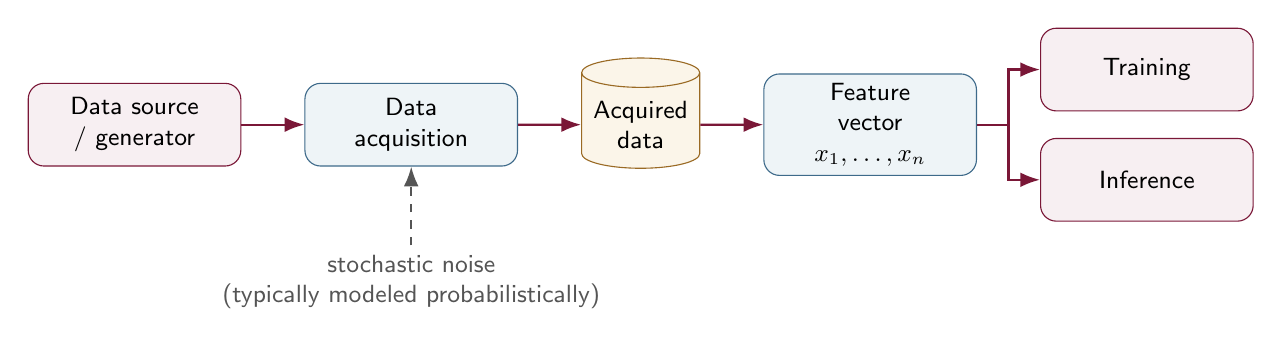
\begin{tikzpicture}[node distance=8mm and 8mm]
\node[systemnode] (source) {Data source\\/ generator};
\node[processnode,right=of source] (acq) {Data\\acquisition};
\node[datastore,right=of acq] (data) {Acquired\\data};
\node[processnode,right=of data] (feat) {Feature\\vector\\$x_1,\ldots,x_n$};
\node[systemnode,right=of feat,yshift=7mm] (train) {Training};
\node[systemnode,right=of feat,yshift=-7mm] (infer) {Inference};
\draw[dataarrow] (source) -- (acq);
\draw[dataarrow] (acq) -- (data);
\draw[dataarrow] (data) -- (feat);
\draw[dataarrow] (feat.east) -- ++(4mm,0) |- (train.west);
\draw[dataarrow] (feat.east) -- ++(4mm,0) |- (infer.west);
\node[below=10mm of acq,align=center,font=\small\sffamily,color=TextSecondary] (noise) {stochastic noise\\(typically modeled probabilistically)};
\draw[controlarrow] (noise) -- (acq.south);
\end{tikzpicture}
\caption{Classical world view: data are generated independently of the model, and acquisition noise is treated as stochastic.}
\label{fig:classical-world}
\end{figure}

The associated assumptions are that the \textbf{source of data does not depend on the model} and that acquisition noise is stochastic in nature, commonly modeled with distributions such as the Gaussian distribution.

\subsection{The adversarial view}

In an adversarial environment, the noise or manipulation is \emph{purposeful}. The attacker can craft data based on knowledge of the model and its behavior.

\begin{figure}[H]
\centering
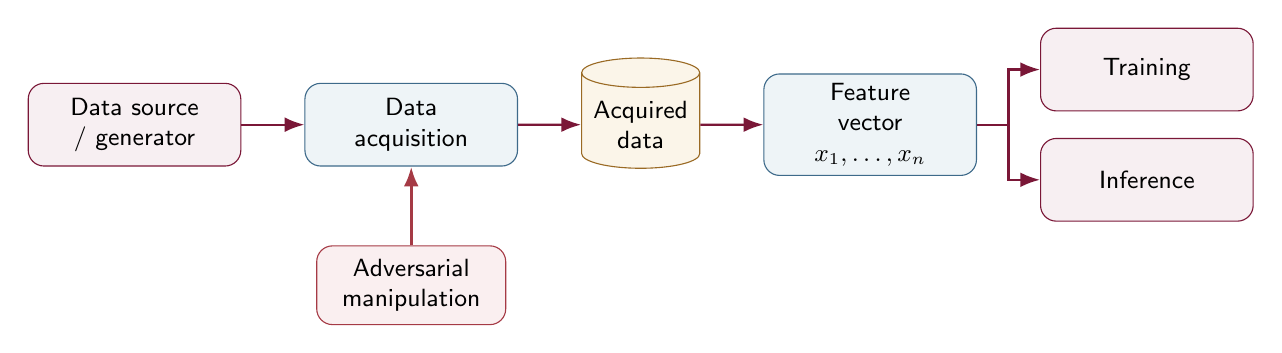
\begin{tikzpicture}[node distance=8mm and 8mm]
\node[systemnode] (source) {Data source\\/ generator};
\node[processnode,right=of source] (acq) {Data\\acquisition};
\node[datastore,right=of acq] (data) {Acquired\\data};
\node[processnode,right=of data] (feat) {Feature\\vector\\$x_1,\ldots,x_n$};
\node[systemnode,right=of feat,yshift=7mm] (train) {Training};
\node[systemnode,right=of feat,yshift=-7mm] (infer) {Inference};
\node[threatnode,below=10mm of acq] (adv) {Adversarial\\manipulation};
\draw[dataarrow] (source) -- (acq);
\draw[dataarrow] (acq) -- (data);
\draw[dataarrow] (data) -- (feat);
\draw[dataarrow] (feat.east) -- ++(4mm,0) |- (train.west);
\draw[dataarrow] (feat.east) -- ++(4mm,0) |- (infer.west);
\draw[-{Latex[length=2.5mm]},very thick,draw=MutedRed] (adv) -- (acq.south);
\end{tikzpicture}
\caption{Adversarial world view: inputs may be deliberately manipulated to influence training or inference.}
\label{fig:adversarial-world}
\end{figure}

\begin{warningbox}[title={Stochastic noise vs. adversarial data}]
Stochastic noise is modeled as random variation. Adversarial data are \textbf{not random}: they are chosen with an objective and often depend on the decision rule, model parameters, available feedback, or other information about the system.
\end{warningbox}

\section{Motivating Example: Spam Filtering}

A simple linear spam classifier shows how knowledge of a decision rule can change the data-generation process. Suppose a message contains the keywords \emph{buy} and \emph{bitcoins}, with weights $2.0$ and $4.0$. The classifier uses a threshold of $5.0$.

\begin{equation}
 s(x)=\sum_{j=1}^{d} w_j x_j.
 \label{eq:spam-score}
\end{equation}
\wherelegend
\begin{itemize}
  \item $x_j$: feature indicating the presence or amount of the $j$-th keyword;
  \item $w_j$: weight assigned to that feature by the classifier;
  \item $d$: number of features;
  \item $s(x)$: classifier score.
\end{itemize}

With \emph{buy} and \emph{bitcoins} present, the score is $2+4=6$, hence $6>5$ and the message is classified as spam. If the attacker inserts the word \emph{uncle}, whose weight in this example is $-2$, the score becomes $2+4-2=4$, so $4<5$ and the same underlying spam message crosses the decision boundary and is classified as non-spam.

\begin{examplebox}[title={Adversarial adaptation}]
The message is not modified by random corruption. It is modified \emph{because} the attacker knows or infers which features reduce the spam score. The data-generation process therefore depends on the model.
\end{examplebox}

\section{The Cybersecurity Arms Race}

Cybersecurity can be viewed as a repeated adversary--defender cycle:

\begin{figure}[H]
\centering
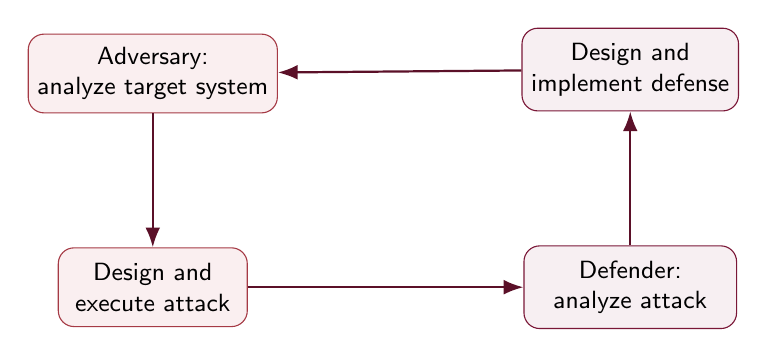
\begin{tikzpicture}[node distance=17mm and 35mm]
\node[threatnode] (a1) {Adversary:\\analyze target system};
\node[threatnode,below=of a1] (a2) {Design and\\execute attack};
\node[systemnode,right=of a2] (d1) {Defender:\\analyze attack};
\node[systemnode,above=of d1] (d2) {Design and\\implement defense};
\draw[arrow] (a1) -- (a2);
\draw[arrow] (a2) -- (d1);
\draw[arrow] (d1) -- (d2);
\draw[arrow] (d2) -- (a1);
\end{tikzpicture}
\caption{Security is an iterative arms race: attacks reveal weaknesses, defenses change the system, and attackers adapt.}
\label{fig:arms-race}
\end{figure}

Three practical rules follow: \textbf{know your adversary}, \textbf{be proactive}, and \textbf{protect your model}.

\section{Threat Modeling}

\begin{definitionbox}
A machine-learning \textbf{threat model} characterizes the adversary along three dimensions:
\begin{enumerate}
  \item \textbf{knowledge}: what the adversary knows about the data, model, and outputs;
  \item \textbf{goal}: what security property the adversary wants to violate;
  \item \textbf{capability}: what the adversary is able to modify or query, and under which constraints.
\end{enumerate}
\end{definitionbox}

\subsection{Adversary's goal: integrity, availability, confidentiality}

Adversarial goals can be mapped to the classical CIA security properties.

\begin{table}[H]
\centering
\caption{Adversarial goals for machine-learning systems.}
\label{tab:cia-ml}
\begin{tabularx}{\textwidth}{>{\bfseries}p{0.20\textwidth}X X}
\toprule
\rowcolor{Primary}
\color{white}Goal & \color{white}Meaning & \color{white}Representative consequence \\
\midrule
Integrity & Compromise the model's intended operation & Deliberately cause samples to be misclassified \\
Availability & Compromise access to, or normal operation of, the model & Errors or behavior that can produce denial of service or prevent normal use \\
Confidentiality & Extract private information from the model & Reveal confidential information about the model or its users \\
\bottomrule
\end{tabularx}
\end{table}

\subsection{Adversary's knowledge}

Adversarial knowledge can concern three major resources: \textbf{training data}, \textbf{model details}, and \textbf{output feedback}. Three broad attack settings are useful:

\begin{table}[H]
\centering
\caption{Knowledge-based attack settings.}
\label{tab:attack-knowledge}
\begin{tabularx}{\textwidth}{>{\bfseries}p{0.19\textwidth}p{0.24\textwidth}X}
\toprule
\rowcolor{Primary}
\color{white}Setting & \color{white}Knowledge & \color{white}Interpretation \\
\midrule
White-box & Perfect / complete & Worst-case scenario for the defender; provides an upper bound on performance degradation under attack. \\
Gray-box & Partial & Typical realistic setting; which information is available depends on the use case. \\
Black-box & No internal model knowledge in the simplified taxonomy used here & Very weak adversarial model and best case for the defender; this extreme is often unrealistic. \\
\bottomrule
\end{tabularx}
\end{table}

\subsection{Kerckhoffs' principle}

\begin{keybox}[title={``The enemy knows the system''}]
A secure system should remain secure even when its design is public. Security should not rely on obscurity. In ML, it is often reasonable to assume that an attacker knows the algorithms being used, has at least partial information about training data, and can infer a rough model architecture. Therefore, an ML model should be tested under \textbf{varying levels of adversarial knowledge and access}.
\end{keybox}

\subsection{Adversary's capability: training time vs. inference time}

Two high-level capability surfaces are emphasized:

\begin{table}[H]
\centering
\caption{Capabilities at training and inference time.}
\label{tab:capabilities}
\begin{tabularx}{\textwidth}{>{\bfseries}p{0.24\textwidth}X X}
\toprule
\rowcolor{Primary}
\color{white}Phase & \color{white}Adversarial capability & \color{white}Representative examples \\
\midrule
Training time & Modify or inject training data so that the learned model contains errors or vulnerabilities that appear later at inference & Poisoning, backdoors, payload injection \\
Inference time & Manipulate samples sent to the trained model or exploit model responses & Evasion attacks, adversarial examples, membership inference \\
\bottomrule
\end{tabularx}
\end{table}

\begin{examplebox}[title={Training-time manipulation: Microsoft Tay}]
Microsoft's Tay chatbot provides a concrete example of a learning system exposed to adversarial user-controlled data. A coordinated group exploited the system shortly after launch and drove it toward inappropriate outputs. The security lesson is broader than the product itself: when a system updates or adapts from user-provided interactions, the training signal becomes part of the attack surface.
\end{examplebox}

\subsection{Capability constraints and the feasible domain}

Attackers are powerful but not unconstrained. Malicious modifications must often remain \emph{valid} and \emph{useful} in the underlying application domain:
\begin{itemize}
  \item phishing emails must still be readable and understandable to humans;
  \item phishing-site images must still resemble the intended original sufficiently to be credible;
  \item malware binaries must remain executable and still perform their malicious function;
  \item an attacker typically does not control every stage of the entire ML pipeline.
\end{itemize}

At training time, the adversary may control only a small fraction of a very large dataset, and may be restricted to adding, removing, or modifying particular points. At inference time, query modifications must stay in the \textbf{feasible domain}: the subset of the input space that satisfies application-specific constraints, such as structural constraints on binary executables.

\begin{warningbox}[title={Do not choose an unrealistic attacker}]
Security analysis should avoid both extremes. Assuming an infinitely strong adversary can make the evaluation uninformative about real deployment, while assuming an unrealistically weak adversary can create a false sense of robustness. Systems should therefore be tested at \textbf{several levels of adversarial capability}.
\end{warningbox}

\begin{takeawaybox}
\begin{itemize}
  \item Classical ML assumes data generation is independent of the model; adversarial ML explicitly breaks that assumption.
  \item Threat modeling requires a clear statement of the adversary's \textbf{knowledge}, \textbf{goal}, and \textbf{capability}.
  \item Integrity, availability, and confidentiality provide a useful taxonomy of attacker objectives.
  \item White-, gray-, and black-box settings differ in how much the attacker knows about the system.
  \item Training-time and inference-time attacks expose different parts of the pipeline.
  \item Real attackers operate under feasibility constraints; robust evaluation should model these constraints rather than ignoring them.
\end{itemize}
\end{takeawaybox}

% =============================================================================
% LECTURE 2
% =============================================================================
\chapter{Basic Machine-Learning Refresher}

\section{Types of Machine Learning}

Three broad learning paradigms are:
\begin{itemize}
  \item \textbf{supervised learning}: task-driven learning from labeled examples, typically for prediction;
  \item \textbf{unsupervised learning}: data-driven learning of structure such as clusters or latent representations;
  \item \textbf{reinforcement learning}: learning from interaction and feedback---informally, learning from the consequences of previous actions.
\end{itemize}

\section{What It Means for a Program to Learn}

Tom M. Mitchell's formulation describes learning through a \textbf{task} $T$, a \textbf{performance measure} $P$, and an \textbf{experience} $E$. A program learns when its measured performance on tasks in $T$ improves with experience $E$.

\subsection{Task}

A machine-learning task is typically one that is difficult to solve by a conventional fixed program. A dataset contains many examples; each example is described through a collection of \textbf{features} and represented as a feature vector
\begin{equation}
  \vect{x} = (x_1,x_2,\ldots,x_n)^\top \in \R^n.
  \label{eq:feature-vector}
\end{equation}
\wherelegend
\begin{itemize}
  \item $\vect{x}$: one example expressed numerically;
  \item $x_i$: the $i$-th feature of the example;
  \item $n$: number of features, i.e. the feature-vector dimensionality.
\end{itemize}

Typical tasks include classification, regression, synthesis/sampling, and probability estimation.

\subsection{Performance measure}

For binary classification, a confusion matrix distinguishes four outcomes:
\begin{itemize}
  \item \textbf{TP}: true positive;
  \item \textbf{TN}: true negative;
  \item \textbf{FP}: false positive;
  \item \textbf{FN}: false negative.
\end{itemize}

\begin{metricbox}[title={Accuracy}]
\begin{equation}
  \mathrm{Accuracy} = \frac{TP+TN}{TP+TN+FP+FN}.
  \label{eq:accuracy}
\end{equation}
\wherelegend
$TP$ and $TN$ are correct predictions, while $FP$ and $FN$ are incorrect predictions. The denominator is the total number of evaluated examples.
\end{metricbox}

Accuracy can be misleading on imbalanced data. If a dataset contains $9900$ negative examples and only $100$ positive examples, a classifier that predicts every sample as negative obtains $99\%$ accuracy while identifying none of the positives.

\begin{metricbox}[title={Precision and Recall}]
\begin{align}
  \mathrm{Precision} &= \frac{TP}{TP+FP}, \label{eq:precision}\\
  \mathrm{Recall} &= \frac{TP}{TP+FN}. \label{eq:recall}
\end{align}
\wherelegend
\begin{itemize}
  \item precision asks: among predicted positives, how many are truly positive?;
  \item recall asks: among truly positive examples, how many were recovered by the model?
\end{itemize}
\end{metricbox}

\subsection{Experience}

In supervised learning, experience is provided by a dataset of labeled examples. Each datapoint $\vect{x}_i$ has a corresponding label $y_i$, which indicates the target class or target value associated with that datapoint.

\section{Features, Feature Space, and Data Representation}

The way data are represented determines which patterns are easy or difficult for a learner to exploit. The same geometric data can look difficult to separate in Cartesian coordinates but much simpler in polar coordinates; a representation change can therefore expose useful structure.

\begin{definitionbox}
A \textbf{feature space} is the coordinate space induced by a chosen representation or transformation of the original feature vector. There is no single universal feature space: its dimensionality and geometry depend on the transformation applied to the data.
\end{definitionbox}

\begin{table}[H]
\centering
\caption{How increasingly data-driven systems obtain representations.}
\begin{tabularx}{\textwidth}{>{\raggedright\arraybackslash\bfseries}p{0.22\textwidth}>{\raggedright\arraybackslash}X>{\raggedright\arraybackslash}X}
\toprule
\rowcolor{Primary}
\color{white}Approach & \color{white}Representation / features & \color{white}Mapping to output \\
\midrule
Rule-based system & Hand-designed representation embedded in the program & Hand-designed rules/program \\
Classical machine learning & Hand-designed or engineered features & Mapping learned from data \\
Representation learning & Features and output mapping are learned from data & Learned mapping \\
Deep learning & Multiple layers learn progressively richer representations & Learned end-to-end mapping \\
\bottomrule
\end{tabularx}
\end{table}

\begin{figure}[H]
\centering
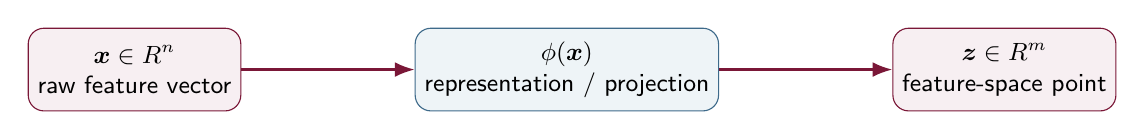
\begin{tikzpicture}[node distance=16mm and 22mm]
\node[systemnode] (x) {$\vect{x}\in\R^n$\\raw feature vector};
\node[processnode,right=of x] (phi) {$\phi(\vect{x})$\\representation / projection};
\node[systemnode,right=of phi] (z) {$\vect{z}\in\R^m$\\feature-space point};
\draw[dataarrow] (x) -- (phi);
\draw[dataarrow] (phi) -- (z);
\end{tikzpicture}
\caption{A feature vector can be transformed into a different feature-space representation. Deep networks learn such transformations internally.}
\label{fig:feature-space}
\end{figure}

Deep neural networks learn feature representations rather than relying only on hand-designed features. Feature-space dimensionality depends on the learned or chosen transformation.

\section{Linear Regression}

Linear regression models the relationship between one or more explanatory variables and a dependent numerical variable. Its prediction rule is
\begin{equation}
  \hat{y} = \vect{w}^{\top}\vect{x} + b.
  \label{eq:linear-regression}
\end{equation}
\wherelegend
\begin{itemize}
  \item $\vect{x}\in\R^n$: input feature vector;
  \item $\vect{w}\in\R^n$: model parameters, also called weights;
  \item $b\in\R$: bias or intercept;
  \item $\hat{y}\in\R$: predicted scalar output.
\end{itemize}

A large-magnitude weight $w_i$ means that feature $x_i$ has a large effect on the linear prediction. A negative $w_i$ means that increasing $x_i$ decreases the prediction, all else being equal.

For a linear-algebra refresher, see: \url{https://www.deeplearningbook.org/contents/linear_algebra.html}.

\subsection{Train, validation, and test sets}

Standard dataset-split terminology:
\begin{itemize}
  \item \textbf{training set}: often around $70\%$--$90\%$ of the dataset, used to fit model parameters;
  \item \textbf{test set}: held out from training and used to evaluate generalization after training;
  \item \textbf{validation set}: optionally held out for selecting hyperparameters during model development.
\end{itemize}

\subsection{Mean squared error}

\begin{metricbox}[title={Mean Squared Error (MSE)}]
\begin{equation}
  \mathrm{MSE} = \frac{1}{m}\sum_{i=1}^{m}\left(\hat{y}_i-y_i\right)^2.
  \label{eq:mse}
\end{equation}
\wherelegend
\begin{itemize}
  \item $m$: number of examples in the evaluated set;
  \item $y_i\in\R$: true target for example $i$;
  \item $\hat{y}_i\in\R$: model prediction for example $i$.
\end{itemize}
The squared term penalizes large errors more strongly than small errors. During training the MSE can be evaluated on training data; after training it can be evaluated on held-out data to assess generalization.
\end{metricbox}

\section{Learning as Optimization}

Learning can be formulated as optimization of an \textbf{objective function} (also called a criterion). A maximization problem can be converted into minimization by negating the objective, so machine-learning training is often written as a minimization problem.

A useful distinction is between \textbf{loss} and \textbf{cost}: the loss refers to the error for one example, while the cost is an average or aggregate over the dataset. In practice, papers sometimes use these terms interchangeably.

For squared error:
\begin{align}
  L(\hat{y},y) &= (\hat{y}-y)^2,\\
  J(\theta) &= \frac{1}{m}\sum_{i=1}^{m}L\bigl(f(\vect{x}_i;\theta),y_i\bigr).
  \label{eq:cost-general}
\end{align}
\wherelegend
\begin{itemize}
  \item $L$: per-example loss;
  \item $J$: dataset-level cost/objective;
  \item $\theta$: all trainable model parameters;
  \item $f(\vect{x}_i;\theta)$: model prediction for example $i$.
\end{itemize}

\section{Gradient-Based Optimization}

\subsection{Derivative and local linear approximation}

For a scalar function $y=f(x)$, the derivative $f'(x)$ gives the instantaneous rate of change. For a sufficiently small perturbation $\epsilon$,
\begin{equation}
  f(x+\epsilon) \approx f(x) + \epsilon f'(x).
  \label{eq:first-order}
\end{equation}
\wherelegend
\begin{itemize}
  \item $x$: current input point;
  \item $\epsilon$: small input perturbation;
  \item $f'(x)$: derivative at $x$.
\end{itemize}
If $f'(x)>0$, moving in the negative direction tends to decrease $f$ locally; if $f'(x)<0$, moving in the positive direction tends to decrease it.

\subsection{Single-variable gradient descent}

A simple descent intuition is to move with the opposite sign of the derivative:
\begin{equation}
  x \leftarrow x - \epsilon\,\mathrm{sign}\bigl(f'(x)\bigr).
  \label{eq:sign-descent}
\end{equation}
This captures the direction of descent. Practical gradient descent typically uses the derivative magnitude as well, as in the multivariable update below.

A point where $f'(x)=0$ is a \textbf{critical point}. Critical points include global minima, local minima, maxima, and saddle points. In high-dimensional optimization, locating a global minimum can be difficult; iterative methods generally seek useful low-loss solutions.

\subsection{Multivariable gradients}

For $f:\R^n\to\R$, the gradient is the vector of partial derivatives:
\begin{equation}
  \nabla f(\vect{x}) =
  \begin{bmatrix}
    \dfrac{\partial f}{\partial x_1}\\[0.45em]
    \vdots\\[0.2em]
    \dfrac{\partial f}{\partial x_n}
  \end{bmatrix}.
  \label{eq:gradient}
\end{equation}
\wherelegend
\begin{itemize}
  \item $\vect{x}\in\R^n$: optimization variable;
  \item $\partial f/\partial x_i$: rate of change with respect to coordinate $x_i$;
  \item $\nabla f(\vect{x})$: direction of steepest local ascent.
\end{itemize}
In multiple dimensions, a differentiable critical point satisfies $\nabla f(\vect{x})=\vect{0}$.

Gradient descent moves in the opposite direction:
\begin{equation}
  \vect{x} \leftarrow \vect{x} - \alpha\nabla f(\vect{x}).
  \label{eq:gradient-descent}
\end{equation}
\wherelegend
$\alpha>0$ is the \textbf{learning rate}, which controls the size of each optimization step.

For ordinary linear regression, the MSE is a convex function of the linear parameters and can be solved directly by setting the gradient to zero. Neural networks generally do not admit a comparable closed-form solution, so iterative optimization is used.

\section{Generalization, Capacity, and Overfitting}

A model can achieve very low training loss while performing poorly on unseen samples. The objective is not to memorize the training set, but to learn a rule that \textbf{generalizes}.

\begin{remarkbox}[title={Overfitting intuition}]
John von Neumann's often-cited warning---``With four parameters I can fit an elephant, and with five I can make him wiggle his trunk''---captures the danger of excessive model flexibility: fitting the observed data is not the same as learning a rule that generalizes.
\end{remarkbox}

\begin{table}[H]
\centering
\caption{Underfitting, appropriate fit, and overfitting.}
\label{tab:fitting}
\begin{tabularx}{\textwidth}{>{\bfseries}p{0.20\textwidth}X X}
\toprule
\rowcolor{Primary}
\color{white}Regime & \color{white}Training behavior & \color{white}Generalization behavior \\
\midrule
Underfitting & Model is too restricted to capture important structure & High training and test error \\
Appropriate fit & Capacity is sufficient without fitting incidental noise & Low error on unseen data \\
Overfitting & Model fits training details/noise too aggressively & Very low training error but worse validation/test error \\
\bottomrule
\end{tabularx}
\end{table}

\textbf{Capacity} is the model family's ability to fit a broad variety of functions. Increasing capacity can reduce underfitting, but excessive capacity can increase overfitting. In a polynomial model, capacity can be increased by adding higher-order features $x,x^2,x^3,\ldots$.

\section{Regularization}

\begin{definitionbox}
\textbf{Regularization} is a modification to the learning procedure intended to reduce generalization error rather than merely reduce training error. It effectively restricts or biases the set of functions the learner prefers.
\end{definitionbox}

Two examples are weight decay and dataset augmentation.

\subsection{Weight decay}

A squared-$\ell_2$ penalty encourages smaller parameter values. A regularized objective can be written as
\begin{equation}
  J(\theta)=\mathrm{MSE}_{\mathrm{train}} + \lambda\lVert\theta\rVert_2^2.
  \label{eq:weight-decay-source}
\end{equation}
\wherelegend
\begin{itemize}
  \item $\theta$: model parameters;
  \item $\lambda\ge 0$: regularization coefficient;
  \item $\lVert\theta\rVert_2^2$: squared Euclidean norm of the parameters.
\end{itemize}

The gradient $\nabla J$ describes the local slope of the objective. The \textbf{Hessian} $H=\nabla^2J$ contains second derivatives, so it describes how the gradient changes and captures the local curvature of the loss surface. Adding an $\ell_2$ penalty contributes a positive diagonal term to this curvature and can make the optimization landscape more well-behaved.

Using the closely related convention $\frac{\lambda}{2}\lVert\theta\rVert_2^2$, the regularizer contributes
\begin{equation}
  \nabla^2\!\left(\frac{\lambda}{2}\lVert\theta\rVert_2^2\right)=\lambda I,
  \qquad
  H = H_{\mathrm{MSE}} + \lambda I.
  \label{eq:weight-decay-hessian}
\end{equation}
\wherelegend
\begin{itemize}
  \item $H$: Hessian of the total objective;
  \item $H_{\mathrm{MSE}}$: Hessian of the unregularized MSE term;
  \item $I$: identity matrix.
\end{itemize}

\begin{remarkbox}[title={Source-notation consistency}]
The source material uses $\lambda\lVert\theta\rVert_2^2$ on one page and $\frac{\lambda}{2}\lVert\theta\rVert_2^2$ when deriving the Hessian on the next. These conventions differ only by a constant factor that can be absorbed into the definition of $\lambda$, but the Hessian equation $\lambda I$ corresponds directly to the latter convention.
\end{remarkbox}

\subsection{Dataset augmentation}

A larger and more representative dataset usually improves generalization, but real data are limited. \textbf{Dataset augmentation} creates additional reasonable examples.
\begin{itemize}
  \item \textbf{Synthetic data}: new examples generated from scratch, potentially by another generative model.
  \item \textbf{Augmented data}: transformations of existing examples $\vect{x}_i$ that preserve the relevant semantics.
\end{itemize}
For images, common augmentation examples here are noise injection, geometric transformations, color transformations, erasure, cropping, flipping, rotation, and brightness adjustment.

\section{Data Normalization}

Features can have very different scales, such as age and income. Large scale differences can skew a DNN's loss surface, slow gradient-based optimization, cause updates to overshoot useful optima or become poorly directed, and increase numerical-instability risk. Normalization rescales features to a comparable range, typically producing a smoother optimization surface and making gradient-based learning easier.

\subsection{Min--max scaling}
\begin{equation}
  x' = \frac{x-x_{\min}}{x_{\max}-x_{\min}}.
  \label{eq:minmax}
\end{equation}
\wherelegend
\begin{itemize}
  \item $x$: original feature value;
  \item $x_{\min}$ and $x_{\max}$: minimum and maximum values used for scaling;
  \item $x'$: rescaled value, typically in $[0,1]$.
\end{itemize}
Min--max scaling is sensitive to outliers.

\subsection{Z-score standardization}
\begin{equation}
  x' = \frac{x-\mu}{\sigma}.
  \label{eq:zscore}
\end{equation}
\wherelegend
\begin{itemize}
  \item $\mu$: feature mean;
  \item $\sigma$: feature standard deviation;
  \item $x'$: standardized value, with approximately zero mean and unit standard deviation when computed over the same dataset.
\end{itemize}

\section{Validation and Cross-Validation}

A validation set is held out during training and used to evaluate the model at intermediate stages, tune hyperparameters such as the learning rate or number of parameters, and detect overfitting. A pattern of high training performance but low validation performance is evidence of poor generalization.

\subsection{K-fold cross-validation}

The data are split into $K$ folds. For each run, the model is trained on $K-1$ folds and evaluated on the remaining fold. The process is repeated until each fold has served as the held-out fold. Depending on the experimental protocol, the held-out fold can support validation/model selection or performance testing/estimation.

\begingroup
\setlength{\intextsep}{8pt}
\captionsetup{skip=4pt}
\begin{figure}[H]
\centering
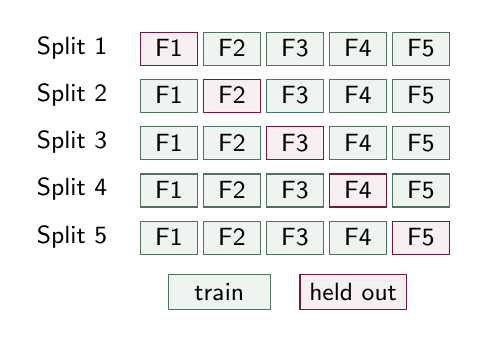
\begin{tikzpicture}[font=\sffamily\small]
\foreach \r in {0,...,4}{
  \node[anchor=east] at (-0.3,-0.60*\r) {Split \the\numexpr\r+1\relax};
  \foreach \c in {0,...,4}{
    \pgfmathtruncatemacro{\isvalid}{\r==\c}
    \ifnum\isvalid=1
      \filldraw[fill=PrimaryLight,draw=Primary] (0.8*\c,-0.60*\r-0.22) rectangle ++(0.72,0.42);
    \else
      \filldraw[fill=MutedGreenLight,draw=MutedGreen] (0.8*\c,-0.60*\r-0.22) rectangle ++(0.72,0.42);
    \fi
    \node at (0.8*\c+0.36,-0.60*\r) {F\the\numexpr\c+1\relax};
  }
}
\node[draw=MutedGreen,fill=MutedGreenLight,minimum width=1.3cm,minimum height=0.45cm] at (1.0,-3.1) {train};
\node[draw=Primary,fill=PrimaryLight,minimum width=1.3cm,minimum height=0.45cm] at (2.7,-3.1) {held out};
\end{tikzpicture}
\caption{Schematic $5$-fold cross-validation. Each fold is held out once.}
\label{fig:kfold}
\end{figure}
\endgroup

Cross-validation often gives a better approximation of model performance, reduces sampling bias, and maximizes data utilization, but it is computationally expensive because training is repeated multiple times.

\begin{takeawaybox}[breakable=false,before skip=4pt]
\begin{itemize}[itemsep=2pt,topsep=2pt,parsep=0pt]
  \item ML examples are represented as feature vectors, and representation strongly affects learnability.
  \item Accuracy alone can be deceptive, especially with class imbalance; precision and recall expose different error modes.
  \item Linear regression predicts with $\hat y=\vect{w}^{\top}\vect{x}+b$ and can be trained by minimizing MSE.
  \item Gradient descent uses local derivative information to iteratively reduce an objective.
  \item Generalization, not training error alone, is the objective; capacity and regularization control the fit/generalization tradeoff.
  \item Validation sets and cross-validation are tools for model selection and reliable performance estimation.
\end{itemize}
\end{takeawaybox}

% =============================================================================
% LECTURE 3
% =============================================================================
\chapter{Decision Trees, Random Forests, and Deep Neural Networks}

\section{Decision Trees}

A decision tree is a hierarchical collection of conditions, also called splits or tests. Conditions are based on the input features and the decision criteria are learned from data. A condition can be \textbf{axis-aligned}, involving one feature, or \textbf{oblique}, involving multiple features.

\begin{figure}[H]
\centering
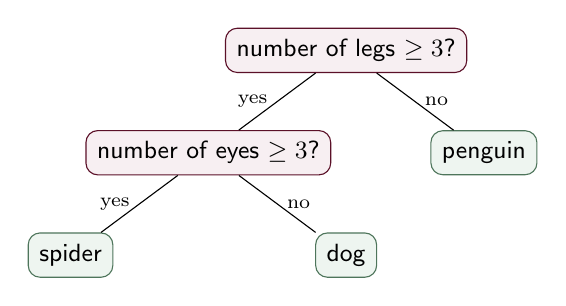
\begin{tikzpicture}[level distance=13mm,sibling distance=35mm]
\node[treecond] {number of legs $\ge 3$?}
  child {node[treecond] {number of eyes $\ge 3$?}
    child {node[treeleaf] {spider} edge from parent node[left,font=\scriptsize]{yes}}
    child {node[treeleaf] {dog} edge from parent node[right,font=\scriptsize]{no}}
    edge from parent node[left,font=\scriptsize]{yes}}
  child {node[treeleaf] {penguin} edge from parent node[right,font=\scriptsize]{no}};
\end{tikzpicture}
\caption{A small binary decision tree: internal nodes evaluate conditions and leaves provide predictions.}
\label{fig:decision-tree}
\end{figure}

Binary decision trees use two-way conditions and are commonly used as the base learners of decision forests such as Random Forests. Non-binary trees can branch into a variable number of conditions, but excessive branching can contribute to overfitting.

\subsection{Training a decision tree}

Finding an optimal decision tree is NP-hard, so practical training relies on heuristic methods such as greedy divide-and-conquer:
\begin{enumerate}
  \item start at the root node;
  \item evaluate candidate conditions;
  \item select the ``best'' condition according to a chosen metric;
  \item recursively repeat the process on the resulting child nodes;
  \item stop when a newly created node contains only, or almost only, samples from one class, i.e. it has high \textbf{purity}.
\end{enumerate}

The set of possible conditions can be very large or even effectively infinite for continuous features, so additional heuristics are used to generate plausible split candidates.

\subsection{Entropy as a purity measure}

Entropy can be used as a measure of class disorder:
\begin{equation}
  H(\vect{p}) = -\sum_{i=1}^{C} p_i\log_2 p_i.
  \label{eq:entropy}
\end{equation}
\wherelegend
\begin{itemize}
  \item $C$: number of classes;
  \item $p_i$: fraction of samples belonging to class $i$ at the node, with $\sum_{i=1}^{C}p_i=1$;
  \item $H$: entropy of the node's class distribution.
\end{itemize}
\begin{notationbox}
The source slide denotes the class fractions by $y_i$. The symbol $p_i$ is used here to avoid confusing class proportions with the target labels $y_i$ used elsewhere in the notes.
\end{notationbox}

Entropy is highest when classes are strongly mixed (for two balanced classes, a $50/50$ mixture) and is minimal when the node contains samples from only one class.

\begin{metricbox}[title={Information Gain}]
Information gain measures the expected reduction in entropy produced by a split on feature $f$:
\begin{equation}
  G(D,f)=H(D)-\sum_{v\in\mathrm{values}(f)}\frac{|D_v|}{|D|}H(D_v).
  \label{eq:information-gain}
\end{equation}
\wherelegend
\begin{itemize}
  \item $D$: set of samples at the current node;
  \item $f$: candidate feature;
  \item $v$: a value of feature $f$;
  \item $D_v\subseteq D$: samples in $D$ whose feature $f$ has value $v$;
  \item $|D_v|/|D|$: relative size of the child subset;
  \item $H(D)$ and $H(D_v)$: parent and child entropies.
\end{itemize}
The second term is the entropy of each possible resulting subset, weighted by its relative size.
\end{metricbox}

For discrete features, candidate values can be evaluated directly and the split with the largest information gain selected. In the simplified treatment used here, continuous features are discretized before applying the same idea. The procedure is then applied recursively until the available selection features or stopping criteria are exhausted.

\section{Ensemble Methods and Random Forests}

\subsection{Ensemble learning}

An ensemble combines multiple classifiers into a single predictor. Each learner estimates the target function, and the individual predictions are aggregated. Combining \textbf{independent and diverse} decisions generally reduces variance and can reduce the final error rate relative to a single model.

\subsection{Random Forest construction}

A Random Forest is an ensemble of decision trees with two principal sources of randomization:
\begin{enumerate}
  \item \textbf{bootstrap sampling}: for each tree, randomly sample training instances with replacement;
  \item \textbf{random feature selection}: at each decision node, choose the best split only from a random subset of $m$ features rather than from all available features. In the source terminology, this is the \textbf{random vector method}.
\end{enumerate}

Each bootstrapped sample is used to train an unpruned decision tree. Samples not selected for a particular bootstrap sample can be used to estimate that tree's error. For prediction, the individual tree outputs are aggregated, usually by majority voting for classification, although weighted aggregation is also possible.

\begin{figure}[H]
\centering
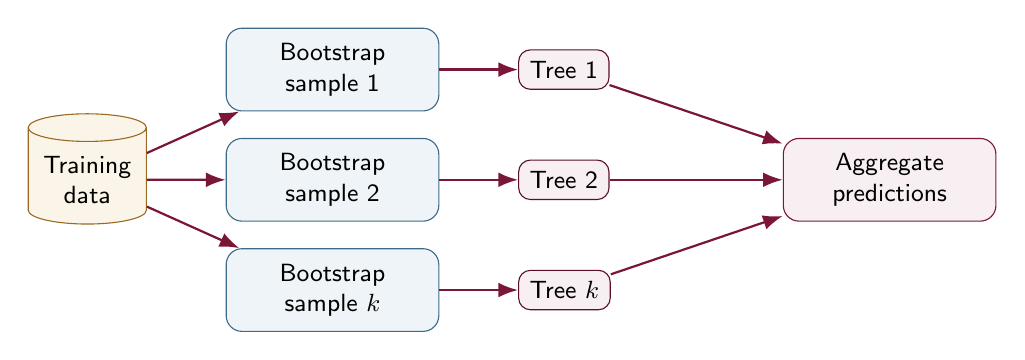
\begin{tikzpicture}[node distance=9mm and 10mm]
\node[datastore] (data) {Training\\data};
\node[processnode,right=of data,yshift=14mm] (b1) {Bootstrap\\sample 1};
\node[processnode,right=of data] (b2) {Bootstrap\\sample 2};
\node[processnode,right=of data,yshift=-14mm] (b3) {Bootstrap\\sample $k$};
\node[treecond,right=of b1] (t1) {Tree 1};
\node[treecond,right=of b2] (t2) {Tree 2};
\node[treecond,right=of b3] (t3) {Tree $k$};
\node[systemnode,right=22mm of t2] (vote) {Aggregate\\predictions};
\draw[dataarrow] (data) -- (b1); \draw[dataarrow] (data) -- (b2); \draw[dataarrow] (data) -- (b3);
\draw[dataarrow] (b1) -- (t1); \draw[dataarrow] (b2) -- (t2); \draw[dataarrow] (b3) -- (t3);
\draw[dataarrow] (t1) -- (vote); \draw[dataarrow] (t2) -- (vote); \draw[dataarrow] (t3) -- (vote);
\end{tikzpicture}
\caption{Random Forest: bootstrapped datasets train diverse trees whose predictions are aggregated. Each tree also uses random feature subsets at its decision nodes.}
\label{fig:random-forest}
\end{figure}

\subsection{Why Random Forests work well}

Random Forests have several useful properties:
\begin{itemize}
  \item bootstrapping and random feature selection promote independence among the decision trees;
  \item greater independence is a key requirement for effective ensembles;
  \item increasing the number of diverse trees is less likely to overfit than repeatedly relying on the same single-tree structure;
  \item predictions depend less strongly on any one specific training sample;
  \item Random Forests are often computationally cheaper than complex neural networks while still performing well on many tasks.
\end{itemize}

\section{Deep Neural Networks}

\subsection{What ``deep'' means}

Deep Neural Network (DNN) is an umbrella term for neural networks with many layers. Examples include deep feedforward networks, convolutional neural networks, recurrent neural networks, generative adversarial networks, and transformer-based neural networks.

The ``neural'' terminology comes from an analogy between an artificial computational unit and a biological neuron: multiple inputs are weighted, combined, and passed through a function that produces an output.

\subsection{Function approximation}

A DNN can be viewed as a function approximator. Suppose the unknown target relationship is
\begin{equation}
  y=f^*(\vect{x}).
  \label{eq:true-function}
\end{equation}
A neural network defines an approximation
\begin{equation}
  \hat y=f(\vect{x};\theta),
  \label{eq:dnn-function}
\end{equation}
\wherelegend
\begin{itemize}
  \item $\vect{x}$: input feature vector;
  \item $f^*$: unknown target function;
  \item $f(\cdot;\theta)$: neural-network approximation parameterized by $\theta$;
  \item $y$: target output and $\hat y$: network prediction.
\end{itemize}
Training adjusts $\theta$ so that $f(\vect{x};\theta)$ approximates $f^*(\vect{x})$ on the relevant data distribution.

\subsection{Feedforward composition and depth}

A feedforward network composes several functions in a directed acyclic graph. For three layers,
\begin{equation}
  f(\vect{x})=f^3\!\left(f^2\!\left(f^1(\vect{x})\right)\right).
  \label{eq:function-composition}
\end{equation}
\wherelegend
\begin{itemize}
  \item $f^1,f^2,f^3$: transformations implemented by consecutive network layers;
  \item the \textbf{depth} of the network is the length of this composition;
  \item feedforward means information moves forward through the directed acyclic computation graph.
\end{itemize}

Training examples provide only inputs and desired outputs. For each datapoint $\vect{x}_i$, the label satisfies conceptually
\begin{equation}
  y_i=f^*(\vect{x}_i),
\end{equation}
and the learning algorithm modifies the hidden-layer parameters so the network output approaches $y_i$.

\section{Representation Learning in Feedforward Networks}

A one-hidden-layer network can be written as a learned nonlinear transformation followed by a linear map:
\begin{equation}
  \hat y=f(\vect{x};\theta,\vect{w})=\phi(\vect{x};\theta)^{\top}\vect{w}.
  \label{eq:phi-model}
\end{equation}
\wherelegend
\begin{itemize}
  \item $\phi(\vect{x};\theta)$: nonlinear representation or feature extractor;
  \item $\theta$: parameters controlling the learned representation;
  \item $\vect{w}$: parameters mapping the learned representation to the output;
  \item $\hat y$: network prediction.
\end{itemize}

This is analogous to linear regression $\hat y=\vect{w}^{\top}\vect{x}+b$, except that the linear mapping is applied to a \emph{learned} representation rather than directly to the raw input. The representation $\phi$ maps the input into an intermediate feature space useful for the task.

The benefit is the ability to learn both a nonlinear feature transformation and an output mapping from a broad family of functions. The cost is that the optimization problem is generally non-convex and lacks a simple closed-form solution.

For compactness, all trainable parameters can be absorbed into a single symbol:
\begin{equation}
  \hat y=f(\vect{x};\theta)=f(\vect{x};W,\phi),
  \label{eq:dnn-notation}
\end{equation}
where $\theta$ denotes all parameters that define the learned network function.

\section{Understanding the Neuron and Activation Function}

\subsection{Weighted inputs and a threshold}

A music-festival decision provides an intuitive neuron example: weather, friends, and transport are features $x_1,x_2,x_3$, their importance is encoded by weights $w_1,w_2,w_3$, and an activation function $g$ converts the weighted combination into a decision.

A threshold unit can be written as
\begin{equation}
  g(\vect{x})=
  \begin{cases}
    1, & \sum_i x_iw_i \ge \text{threshold},\\
    0, & \sum_i x_iw_i < \text{threshold}.
  \end{cases}
  \label{eq:threshold-unit}
\end{equation}
Equivalently, by absorbing the threshold into a bias $b$,
\begin{equation}
  g(\vect{x})=
  \begin{cases}
    1, & \vect{w}^{\top}\vect{x}+b \ge 0,\\
    0, & \vect{w}^{\top}\vect{x}+b < 0.
  \end{cases}
  \label{eq:threshold-bias}
\end{equation}
\wherelegend
\begin{itemize}
  \item $\vect{x}$: input features;
  \item $\vect{w}$: feature weights;
  \item $b$: bias, which shifts the threshold;
  \item $g$: activation/decision function.
\end{itemize}

Changing $\vect{w}$ changes the relative importance of the features. In modern neural networks, the activation is usually a differentiable or piecewise-differentiable nonlinear function rather than a hard threshold.

\subsection{Activation functions}

Let
\begin{equation}
  z=\vect{w}^{\top}\vect{x}+b.
  \label{eq:preactivation}
\end{equation}
\wherelegend
$\vect{x}$ is the input, $\vect{w}$ the weight vector, $b$ the bias, and $z$ the scalar pre-activation. The activation function $g$ maps $z$ to the neuron's output.

\subsubsection{Linear activation}
Consider the simplified linear activation $g(z)=\lambda z$. With $z=\vect{w}^{\top}\vect{x}+b$,
\begin{equation}
  \hat y=g(z)=\lambda\left(\vect{w}^{\top}\vect{x}+b\right).
\end{equation}
If every layer uses only linear activations, the entire composition remains linear. Therefore, multiple layers do not create a richer nonlinear function family.

\subsubsection{Sigmoid}
\begin{equation}
  \sigma(z)=\frac{1}{1+e^{-z}}.
  \label{eq:sigmoid}
\end{equation}
The sigmoid smoothly approximates a step and maps real-valued inputs to $(0,1)$. Its smoothness makes it useful for illustrating gradient-based learning and backpropagation.

\subsubsection{ReLU}
\begin{equation}
  \mathrm{ReLU}(z)=\max\{0,z\}.
  \label{eq:relu}
\end{equation}
ReLU is piecewise linear and widely used in feedforward networks. It preserves simple gradient behavior over its active region while introducing nonlinearity into the overall composition.

\subsubsection{Softmax}
For a vector of logits $\vect{z}$, the softmax output for coordinate $i$ is
\begin{equation}
  \mathrm{softmax}(\vect{z})_i=\frac{e^{z_i}}{\sum_j e^{z_j}}.
  \label{eq:softmax}
\end{equation}
\wherelegend
\begin{itemize}
  \item $z_i$: score/logit for class $i$;
  \item the denominator sums exponentiated scores over all classes;
  \item the output vector is normalized and can be interpreted as a probability distribution.
\end{itemize}
Softmax is therefore useful for multi-class classification outputs.

\begin{figure}[H]
\centering
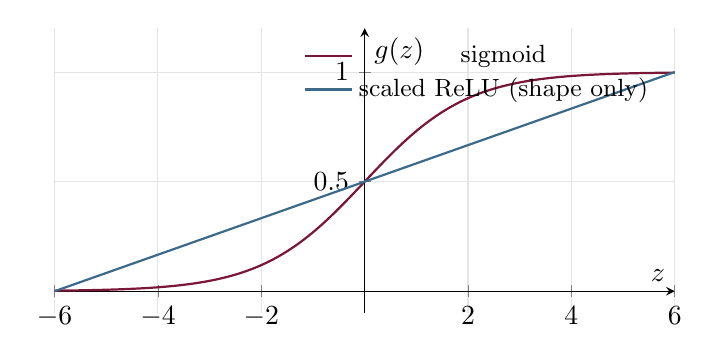
\begin{tikzpicture}
\begin{axis}[width=0.78\textwidth,height=5.2cm,axis lines=middle,xlabel={$z$},ylabel={$g(z)$},xmin=-6,xmax=6,ymin=-0.1,ymax=1.2,grid=both,grid style={draw=SoftGray},legend style={draw=none,fill=none,font=\small}]
\addplot[domain=-6:6,samples=150,thick,draw=Primary] {1/(1+exp(-x))};
\addlegendentry{sigmoid}
\addplot[domain=-6:6,samples=2,thick,draw=MutedBlue] {max(0,x)/6};
\addlegendentry{scaled ReLU (shape only)}
\end{axis}
\end{tikzpicture}
\caption{Schematic activation-function shapes. ReLU is scaled only to share the panel; the analytic definition in \cref{eq:relu} is authoritative.}
\label{fig:activation-shapes}
\end{figure}

\section{Forward Propagation}

A layer first computes an affine transformation and then applies an activation:
\begin{align}
  \vect{z}^{\,i} &= W^i\vect{a}^{\,i-1}+\vect{b}^{\,i},\\
  \vect{a}^{\,i} &= g\!\left(\vect{z}^{\,i}\right).
  \label{eq:layer-forward}
\end{align}
\wherelegend
\begin{itemize}
  \item $i$: layer index;
  \item $W^i$: weight matrix of layer $i$;
  \item $\vect{b}^{\,i}$: bias vector of layer $i$;
  \item $\vect{a}^{\,i-1}$: activations from the previous layer, with $\vect{a}^{\,0}=\vect{x}$;
  \item $\vect{z}^{\,i}$: pre-activation vector;
  \item $\vect{a}^{\,i}$: activation vector.
\end{itemize}

For a two-layer example:
\begin{align}
  \vect{z}^{\,1} &= W^1\vect{x}+\vect{b}^{\,1}, & \vect{a}^{\,1}&=\sigma(\vect{z}^{\,1}),\\
  \vect{z}^{\,2} &= W^2\vect{a}^{\,1}+\vect{b}^{\,2}, & \hat y=\vect{a}^{\,2}&=\sigma(\vect{z}^{\,2}).
  \label{eq:two-layer-forward}
\end{align}

\begin{examplebox}[title={Dimension check for the worked forward pass}]
Using the column-vector convention of \cref{eq:layer-forward}, let $\vect{x}\in\R^3$, use three hidden units, and produce one scalar output. Then
\[
W^1\in\R^{3\times 3},\quad \vect{b}^{\,1}\in\R^3,\quad
\vect{z}^{\,1},\vect{a}^{\,1}\in\R^3,
\]
\[
W^2\in\R^{1\times 3},\quad b^2\in\R,\quad
z^2,a^2=\hat y\in\R.
\]
Thus $W^1\vect{x}$ is a $3$-vector and $W^2\vect{a}^{\,1}$ is a scalar. The source slide displays an equivalent row-vector/transposed convention for some shapes; this document uses column vectors consistently throughout.
\end{examplebox}

\begin{figure}[H]
\centering
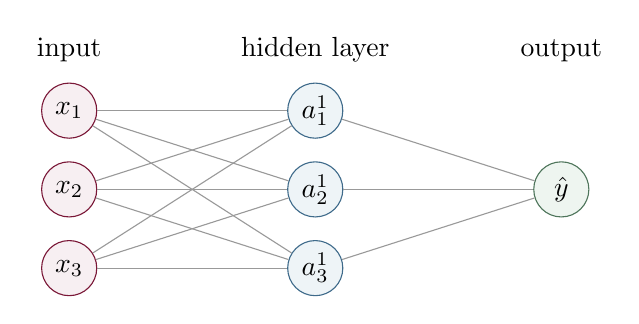
\begin{tikzpicture}[x=1.25cm,y=1.0cm]
\node[inputnode] (i1) at (0,1.5) {$x_1$};
\node[inputnode] (i2) at (0,0.5) {$x_2$};
\node[inputnode] (i3) at (0,-0.5) {$x_3$};
\node[nnnode] (h1) at (2.5,1.5) {$a^1_1$};
\node[nnnode] (h2) at (2.5,0.5) {$a^1_2$};
\node[nnnode] (h3) at (2.5,-0.5) {$a^1_3$};
\node[outputnode] (o) at (5,0.5) {$\hat y$};
\foreach \a in {1,2,3}{\foreach \b in {1,2,3}{\draw[draw=TextSecondary!60] (i\a) -- (h\b);}}
\foreach \b in {1,2,3}{\draw[draw=TextSecondary!60] (h\b) -- (o);}
\node[above] at (0,2.0) {input}; \node[above] at (2.5,2.0) {hidden layer}; \node[above] at (5,2.0) {output};
\end{tikzpicture}
\caption{Forward propagation computes each layer from the previous layer until the network output $\hat y$ is obtained.}
\label{fig:forward-network}
\end{figure}

\section{Gradient Descent for Neural Networks}

The network parameters $\theta$ consist of all weight matrices and bias vectors. For a dataset-level objective
\begin{equation}
  J(\theta)=\frac{1}{m}\sum_{i=1}^{m}L\bigl(f(\vect{x}_i;\theta),y_i\bigr),
  \label{eq:dnn-cost}
\end{equation}
we iteratively update parameters in the direction that reduces the objective:
\begin{equation}
  \theta \leftarrow \theta-\alpha\nabla_{\theta}J(\theta).
  \label{eq:dnn-gd}
\end{equation}
\wherelegend
\begin{itemize}
  \item $m$: number of examples used to evaluate the objective;
  \item $L$: per-example loss;
  \item $\theta$: all network parameters;
  \item $\alpha$: learning rate.
\end{itemize}

For an individual layer $i$, define
\begin{align}
  dW^i &= \frac{\partial J}{\partial W^i}, & d\vect{b}^{\,i} &= \frac{\partial J}{\partial \vect{b}^{\,i}},\\
  W^i &\leftarrow W^i-\alpha dW^i, & \vect{b}^{\,i} &\leftarrow \vect{b}^{\,i}-\alpha d\vect{b}^{\,i}.
  \label{eq:layer-updates}
\end{align}
\wherelegend
$dW^i$ and $d\vect{b}^{\,i}$ denote the gradients of the objective with respect to the weights and biases of layer $i$; $\alpha$ is the learning rate.

\section{Backpropagation}

Backpropagation efficiently computes the gradients needed by \cref{eq:layer-updates}. The chain-rule argument can be organized into four central relationships.

\subsection{Error at the output layer}

For a network with $N$ layers, $\vect{a}^{\,i}=g(\vect{z}^{\,i})$ and $\hat{\vect{y}}=\vect{a}^{\,N}$. The error with respect to the final pre-activation is
\begin{equation}
  d\vect{z}^{\,N}
  =\nabla_{\vect{z}^{\,N}}J
  =\nabla_{\vect{a}^{\,N}}J\,
    \frac{\partial \vect{a}^{\,N}}{\partial \vect{z}^{\,N}}.
  \label{eq:backprop1}
\end{equation}
\wherelegend
\begin{itemize}
  \item $\nabla_{\vect{a}^{\,N}}J$: gradient of the objective with respect to the network output;
  \item $\partial \vect{a}^{\,N}/\partial \vect{z}^{\,N}$: Jacobian of the output activation function;
  \item $d\vect{z}^{\,N}$: output-layer error signal with respect to the pre-activation.
\end{itemize}

The \textbf{Jacobian} generalizes a gradient to a vector-valued function $g:\R^n\to\R^m$; it is the matrix containing all partial derivatives of the outputs with respect to the inputs.

\subsection{Propagating error to an earlier layer}

Recall that
\begin{equation}
  \vect{z}^{\,i+1}=W^{i+1}\vect{a}^{\,i}+\vect{b}^{\,i+1}.
\end{equation}
Using the affine relation above,
\begin{equation}
  d\vect{a}^{\,i}
  =\nabla_{\vect{a}^{\,i}}J
  =\left(W^{i+1}\right)^{\top}d\vect{z}^{\,i+1}.
  \label{eq:backprop2}
\end{equation}
Intuitively, the error at layer $i$ is obtained by transporting the downstream error backward through the weights that connect layer $i$ to layer $i+1$.

Combining \cref{eq:backprop2} with the Jacobian of the activation at layer $i$ gives $d\vect{z}^{\,i}$, and the process repeats backward until the first hidden layer.

\subsection{Weight and bias gradients}

Once $d\vect{z}^{\,i}$ is known,
\begin{align}
  dW^i &= d\vect{z}^{\,i}\left(\vect{a}^{\,i-1}\right)^{\top},
  \label{eq:backprop3}\\
  d\vect{b}^{\,i} &= d\vect{z}^{\,i}.
  \label{eq:backprop4}
\end{align}
\wherelegend
\begin{itemize}
  \item $dW^i$: gradient of the objective with respect to the layer-$i$ weights;
  \item $d\vect{b}^{\,i}$: gradient with respect to the layer-$i$ bias;
  \item $\vect{a}^{\,i-1}$: input activation vector to layer $i$.
\end{itemize}

\begin{figure}[H]
\centering
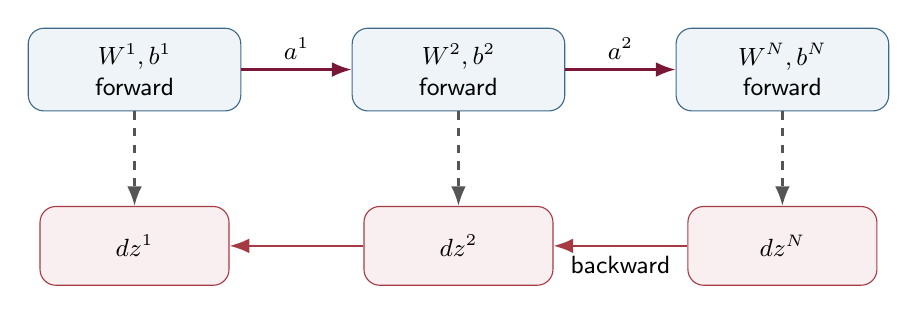
\begin{tikzpicture}[node distance=8mm and 14mm,font=\sffamily\small]
\node[processnode] (l1) {$W^1,b^1$\\forward};
\node[processnode,right=of l1] (l2) {$W^2,b^2$\\forward};
\node[processnode,right=of l2] (ln) {$W^N,b^N$\\forward};
\draw[dataarrow] (l1) -- node[above]{${a}^1$} (l2);
\draw[dataarrow] (l2) -- node[above]{${a}^2$} (ln);
\node[threatnode,below=12mm of ln] (eN) {$d z^N$};
\node[threatnode,below=12mm of l2] (e2) {$d z^2$};
\node[threatnode,below=12mm of l1] (e1) {$d z^1$};
\draw[-{Latex[length=2.5mm]},thick,draw=MutedRed] (eN) -- node[below]{backward} (e2);
\draw[-{Latex[length=2.5mm]},thick,draw=MutedRed] (e2) -- (e1);
\draw[controlarrow] (ln) -- (eN); \draw[controlarrow] (l2) -- (e2); \draw[controlarrow] (l1) -- (e1);
\end{tikzpicture}
\caption{Backpropagation computes output error first and then propagates derivative information backward through the network.}
\label{fig:backprop}
\end{figure}

\begin{keybox}[title={Backpropagation summary}]
The four central relationships are:
\begin{align*}
  d\vect{z}^{\,N} &= \nabla_{\vect{a}^{\,N}}J\,\frac{\partial\vect{a}^{\,N}}{\partial\vect{z}^{\,N}},\\
  d\vect{a}^{\,i} &= (W^{i+1})^{\top}d\vect{z}^{\,i+1},\\
  dW^i &= d\vect{z}^{\,i}(\vect{a}^{\,i-1})^{\top},\\
  d\vect{b}^{\,i} &= d\vect{z}^{\,i}.
\end{align*}
They are an application of the chain rule to the layered computation graph.
\end{keybox}

\section{Stochastic Gradient Descent}

Computing gradients over a very large entire dataset at every update can be prohibitively expensive.

\begin{notationbox}[title={Gradient-descent terminology}]
\textbf{Full-batch gradient descent} uses the entire training set for one update. \textbf{Pure stochastic gradient descent} uses one example per update. The procedure used here samples a subset of examples and is therefore \textbf{mini-batch SGD}, the standard practical variant for neural-network training.
\end{notationbox}

The mini-batch procedure is:
\begin{enumerate}
  \item randomly select a subset of the training data, called a \textbf{mini-batch}, of size $m$;
  \item compute gradients for the examples in the mini-batch;
  \item update weights and biases;
  \item continue until the training data have been traversed;
  \item repeat for the desired number of \textbf{epochs}.
\end{enumerate}

\begin{definitionbox}[title={Epoch and mini-batch}]
A \textbf{mini-batch} is the subset of examples used for one gradient computation/update. An \textbf{epoch} is one traversal of the training dataset under the batching scheme.
\end{definitionbox}

\section{Loss Functions}

Common losses include MSE, binary cross-entropy, cross-entropy, contrastive/triplet losses, and Kullback--Leibler divergence. The first three are developed here; contrastive/triplet losses and KL divergence are listed for completeness but are not developed further.

\subsection{Mean Squared Error}

For regression:
\begin{equation}
  \mathrm{MSE}=\frac{1}{m}\sum_{i=1}^{m}(\hat y_i-y_i)^2.
  \label{eq:dnn-mse}
\end{equation}
\wherelegend
\begin{itemize}
  \item $m$: number of evaluated examples;
  \item $y_i$: true target for example $i$;
  \item $\hat y_i$: prediction for example $i$.
\end{itemize}
MSE penalizes large errors more strongly because the error is squared.

\subsection{Binary cross-entropy}

For binary classification,
\begin{equation}
  \mathcal{L}_{\mathrm{BCE}}
  =-\left[y\log(\hat y)+(1-y)\log(1-\hat y)\right].
  \label{eq:bce}
\end{equation}
\wherelegend
\begin{itemize}
  \item $y\in\{0,1\}$: true binary label;
  \item $\hat y\in(0,1)$: predicted probability of class $1$;
  \item $1-\hat y$: predicted probability of class $0$.
\end{itemize}
BCE is naturally paired with a sigmoid output layer so that the prediction lies in $(0,1)$ and can be interpreted as a Bernoulli probability.

\begin{figure}[H]
\centering
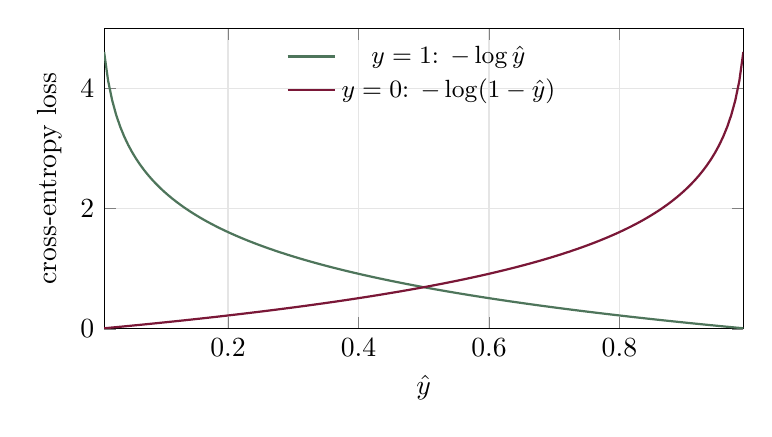
\begin{tikzpicture}
\begin{axis}[width=0.8\textwidth,height=5.4cm,xlabel={$\hat y$},ylabel={cross-entropy loss},xmin=0.01,xmax=0.99,ymin=0,ymax=5,grid=both,grid style={draw=SoftGray},legend style={draw=none,fill=none,font=\small,at={(0.5,0.98)},anchor=north}]
\addplot[domain=0.01:0.99,samples=160,thick,draw=MutedGreen] {-ln(x)};
\addlegendentry{$y=1$: $-\log \hat y$}
\addplot[domain=0.01:0.99,samples=160,thick,draw=Primary] {-ln(1-x)};
\addlegendentry{$y=0$: $-\log(1-\hat y)$}
\end{axis}
\end{tikzpicture}
\caption{Binary cross-entropy penalizes confident wrong predictions sharply. These curves follow \cref{eq:bce} exactly.}
\label{fig:bce-curves}
\end{figure}

\subsection{Multi-class cross-entropy}

For $C$ classes,
\begin{equation}
  \mathcal{L}_{\mathrm{CE}}=-\sum_{i=1}^{C} y_i\log(\hat y_i).
  \label{eq:cross-entropy}
\end{equation}
\wherelegend
\begin{itemize}
  \item $C$: number of classes;
  \item $y_i$: target probability/indicator for class $i$;
  \item $\hat y_i$: predicted probability for class $i$.
\end{itemize}
Multi-class cross-entropy is naturally paired with a softmax output layer, which produces a normalized class-probability vector.

\begin{takeawaybox}
\begin{itemize}
  \item Decision-tree learning greedily chooses splits that increase class purity; entropy and information gain provide one split criterion.
  \item Random Forests combine bootstrap sampling and random feature subsets to create diverse trees and reduce variance.
  \item A DNN is a composition of many parameterized transformations; hidden layers learn intermediate representations.
  \item Nonlinear activation functions are essential: a composition of only linear layers is still linear.
  \item Forward propagation computes activations; backpropagation applies the chain rule to compute gradients layer by layer in reverse.
  \item Mini-batch stochastic gradient descent makes large-scale neural-network optimization computationally feasible.
  \item The output activation and loss function should match the task: MSE for regression, sigmoid+BCE for binary classification, and softmax+cross-entropy for multi-class classification.
\end{itemize}
\end{takeawaybox}

% =============================================================================
% APPENDICES
% =============================================================================
\appendix
\renewcommand{\chapterprefix}{Appendix}
\chapter{Notation and Quick Reference}

\section{Core Symbols}
\begin{table}[H]
\centering
\caption{Notation used throughout the notes.}
\begin{tabularx}{\textwidth}{>{\bfseries}p{0.20\textwidth}X}
\toprule
\rowcolor{Primary}
\color{white}Symbol & \color{white}Meaning \\
\midrule
$\vect{x}$ & Input feature vector \\
$y$ & True target / label \\
$\hat y$ & Model prediction \\
$\vect{w},W$ & Weight vector / weight matrix \\
$b,\vect{b}$ & Bias scalar / bias vector \\
$\theta$ & Collection of trainable model parameters \\
$L$ & Per-example loss \\
$J$ & Dataset-level objective / cost \\
$\alpha$ & Learning rate \\
$\nabla$ & Gradient operator \\
$\phi$ & Learned or chosen feature transformation \\
$\vect{z}^{\,i}$ & Pre-activation at layer $i$ \\
$\vect{a}^{\,i}$ & Activation at layer $i$ \\
\bottomrule
\end{tabularx}
\end{table}

\section{Formula Summary}
\begin{align*}
\text{Linear regression:}\quad & \hat y=\vect{w}^{\top}\vect{x}+b\\
\text{MSE:}\quad & \mathrm{MSE}=\frac{1}{m}\sum_i(\hat y_i-y_i)^2\\
\text{Gradient descent:}\quad & \theta\leftarrow\theta-\alpha\nabla_\theta J\\
\text{Entropy:}\quad & H=-\sum_i p_i\log_2 p_i\\
\text{Information gain:}\quad & G(D,f)=H(D)-\sum_v\frac{|D_v|}{|D|}H(D_v)\\
\text{Sigmoid:}\quad & \sigma(z)=\frac{1}{1+e^{-z}}\\
\text{ReLU:}\quad & \mathrm{ReLU}(z)=\max\{0,z\}\\
\text{Softmax:}\quad & \mathrm{softmax}(\vect{z})_i=\frac{e^{z_i}}{\sum_j e^{z_j}}\\
\text{BCE:}\quad & \mathcal{L}_{\mathrm{BCE}}=-\left[y\log\hat y+(1-y)\log(1-\hat y)\right]\\
\text{Cross-entropy:}\quad & \mathcal{L}_{\mathrm{CE}}=-\sum_i y_i\log\hat y_i.
\end{align*}

\chapter{Glossary}
\begin{description}[style=multiline,leftmargin=3.6cm,labelwidth=3.15cm,labelsep=0.35cm]
\item[Adversarial example] An input deliberately manipulated to induce undesired model behavior while remaining feasible for the application.
\item[Backpropagation] Reverse-mode application of the chain rule used to compute neural-network parameter gradients.
\item[Black-box attack] In the simplified taxonomy used here, an attack with no internal model knowledge.
\item[Capacity] Ability of a model family to represent a wide variety of functions.
\item[Epoch] One traversal of the training dataset under the current batching procedure.
\item[Feature] Measurable or derived component used to represent an example.
\item[Feature space] Space induced by a chosen or learned representation of feature vectors.
\item[Gray-box attack] Attack with partial knowledge of the target system.
\item[Information gain] Expected reduction in entropy resulting from a candidate decision-tree split.
\item[Mini-batch] Subset of training examples used for one gradient computation/update.
\item[Overfitting] Learning training-specific detail that does not generalize well to unseen samples.
\item[Poisoning] Training-time manipulation of learning data intended to alter the resulting model.
\item[Regularization] Modification of a learning procedure intended to reduce generalization error.
\item[Threat model] Explicit specification of adversarial knowledge, goals, and capabilities.
\item[White-box attack] Attack under perfect or near-perfect knowledge of the target model and relevant data in the simplified taxonomy used here.
\end{description}

\chapter{Source Coverage Map}
This appendix records the result of the final completeness audit. Slide ranges refer to the three supplied source PDFs. Status refers to \emph{substantive intellectual content}: title-only slides, repeated screenshots, and decorative examples may be condensed when their security or ML lesson is already represented explicitly.

\subsection*{Course Intro / Threat Modeling}
\begin{table}[H]
\centering
\small
\renewcommand{\arraystretch}{1.12}
\begin{tabularx}{\textwidth}{>{\raggedright\arraybackslash}p{0.11\textwidth}>{\raggedright\arraybackslash}p{0.25\textwidth}>{\raggedright\arraybackslash}X}
\toprule
\rowcolor{Primary}
\color{white}Slides & \color{white}Status & \color{white}Representation in these notes \\
\midrule
1--9 & Fully represented & Orientation, logistics, assessment, and tentative syllabus. \\
10--21 & Condensed / visual content summarized & Voice assistants, autonomous driving, adversarial traffic signs/audio, LLM jailbreaks, prompt injection, browser/agent risks, and economic asymmetry are preserved in prose. \\
22--31 & Fully represented / recreated diagrams & Classical vs. adversarial world models, assumptions, and the spam-classifier example. \\
32--34 & Fully represented / recreated diagram & Adversarial world model, arms race, and key rules. \\
35--43 & Fully represented & Threat-model dimensions, CIA goals, white/gray/black-box knowledge, and Kerckhoffs' principle. \\
44--52 & Fully represented & Training/inference capabilities, Microsoft Tay, feasibility constraints, and realistic capability levels. \\
\bottomrule
\end{tabularx}
\end{table}

\subsection*{Basic ML Refresher}
\begin{table}[H]
\centering
\small
\renewcommand{\arraystretch}{1.12}
\begin{tabularx}{\textwidth}{>{\raggedright\arraybackslash}p{0.11\textwidth}>{\raggedright\arraybackslash}p{0.25\textwidth}>{\raggedright\arraybackslash}X}
\toprule
\rowcolor{Primary}
\color{white}Slides & \color{white}Status & \color{white}Representation in these notes \\
\midrule
1--9 & Fully represented & ML paradigms, $T/P/E$, task types, confusion-matrix outcomes, accuracy, precision, recall, and experience. \\
10--14 & Condensed / recreated diagram & Representation, Cartesian/polar intuition, feature-space projection, and learned features. \\
15--20 & Fully represented & Linear regression, weights/bias, train/validation/test terminology, and MSE. \\
21--31 & Fully represented & Objective/loss/cost, derivatives, critical points, gradients, learning rate, and linear-regression learning. \\
32--37 & Condensed / visual examples summarized & Overfitting/underfitting, generalization, and capacity; illustrative plots are summarized rather than copied. \\
38--43 & Fully represented / visual examples summarized & Regularization, $\ell_2$ weight decay with Hessian intuition, and dataset augmentation. \\
44--47 & Fully represented / recreated diagram & Normalization, validation, and $K$-fold cross-validation. \\
\bottomrule
\end{tabularx}
\end{table}

\subsection*{Decision Trees, RFs, and DNNs}
\begin{table}[H]
\centering
\small
\renewcommand{\arraystretch}{1.12}
\begin{tabularx}{\textwidth}{>{\raggedright\arraybackslash}p{0.11\textwidth}>{\raggedright\arraybackslash}p{0.25\textwidth}>{\raggedright\arraybackslash}X}
\toprule
\rowcolor{Primary}
\color{white}Slides & \color{white}Status & \color{white}Representation in these notes \\
\midrule
1--9 & Fully represented / recreated diagram & Decision trees, binary/non-binary branching, training, entropy, and information gain. \\
10--14 & Fully represented / recreated diagram & Ensemble learning and Random Forest construction/advantages. \\
15--28 & Condensed / recreated concepts & DNN overview, biological analogy, function approximation, feedforward composition, representation learning, and notation. \\
29--37 & Fully represented / recreated plot & Neuron intuition, thresholds/biases, linear activation, sigmoid, ReLU, and softmax. \\
38--45 & Fully represented / worked dimension check & Forward propagation, parameter shapes, objective, and gradient-descent updates. \\
46--53 & Fully represented / recreated diagram & Chain-rule backpropagation, output error, Jacobian, hidden-layer error, $dW$, and $db$. \\
54--61 & Fully represented / recreated plot & Mini-batch SGD, epoch definition, MSE, BCE, cross-entropy, and the additional loss names listed in the source. \\
\bottomrule
\end{tabularx}
\end{table}

\end{document}
